\documentclass[a4paper,11pt]{amsbook}
\usepackage{amsmath}
\usepackage{fullpage}
\usepackage{ tipa }
\pagestyle{headings}
\usepackage{../HBSuerDemir}
\usepackage{graphicx}
\graphicspath{{./ images/ }}
\usepackage{float}

\begin{document}

\hPage{b2p1/212}
The cross sections of EP and HP for $x=k$ or $y=k$ are\\
parabolas and ellipses (hyperbolas) for $z=k$ in EP (HP). Since\\
sections are parabolas in two ways are called \underline{paraboloids}. The\\
third cross sections in EP(HP) being ellipses(hyperbolas) they\\
are respectively called \underline{elliptic paraboloid} (EP),\underline{hyperbolic} \\
\underline{paraboloid} (HP).
\\

\begin{figure}[h]
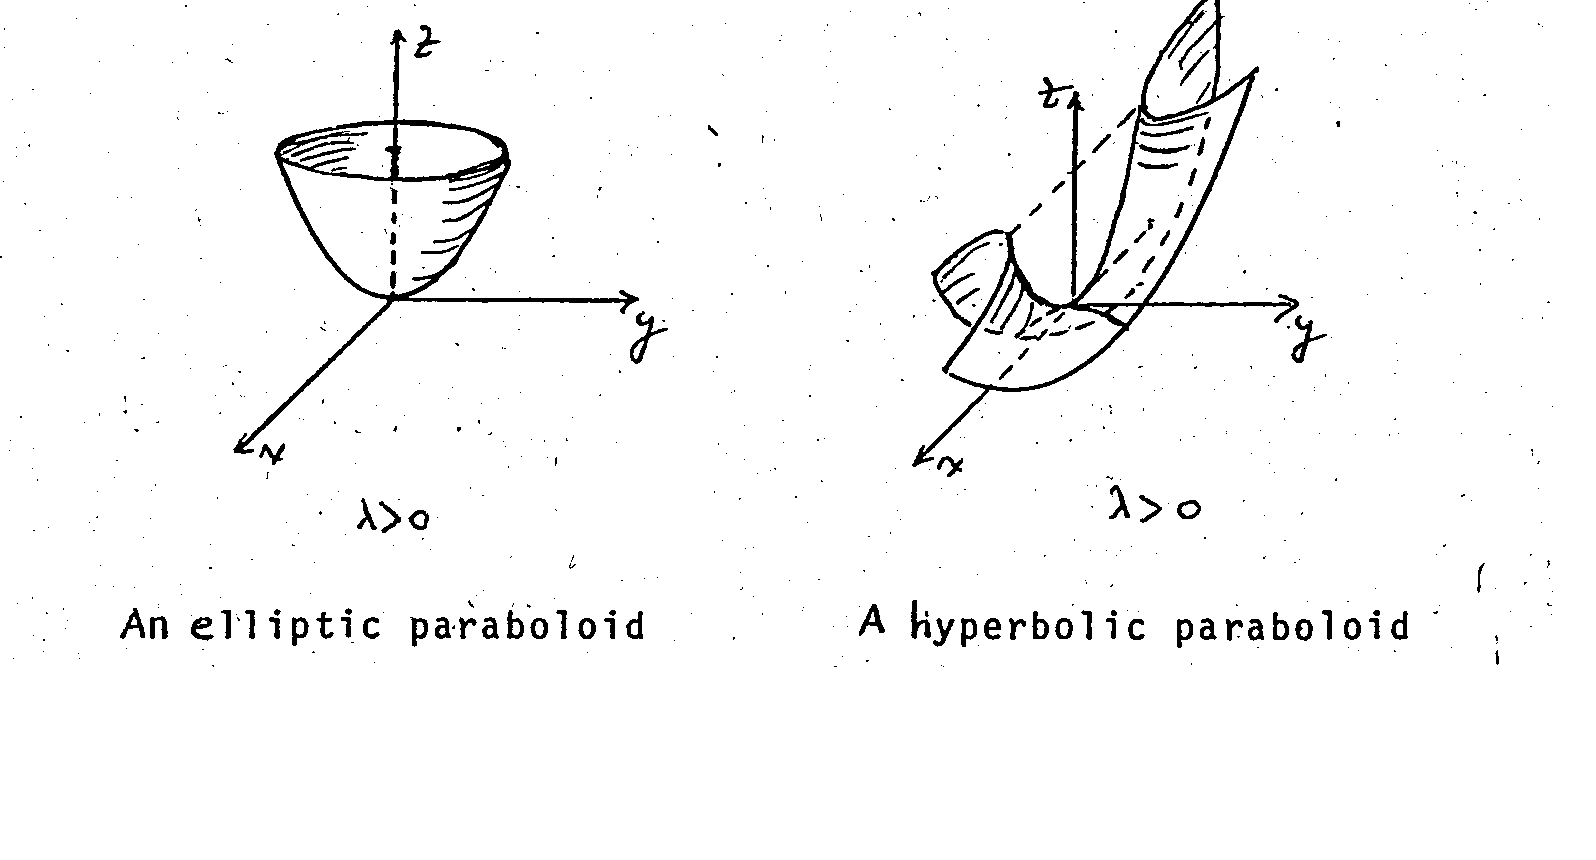
\includegraphics [keepaspectratio=true,scale=0.35]{images/p212-fig1}

\end{figure}

The origin in $H_{1}$ abd $H_{2}$ is called \underline{vertex}. The\\
hyperbolic paraboloid is of saddle shape in the neighborhood of\\
the origin and the origin is called the \underline{saddle point} of the sur-\\
face, and the surface $H_{2}$ is sometimes called a \underline{saddle shape sure-}\\
\underline{face}.\\
\\
Similar results are obtained when $x$ or $y$ are linear\\
instead of $z$.\\
The equations\\
\\
$$\frac{(x-h)^{2}}{a^{2}}\pm\frac{(y-k)^{2}}{b^{2}}=\lambda(z-l)$$\\
\\
represent clearly paraboloids having vertex at $(h,k,z)$.\\
\\
\begin{exmp}
Sketch\\
\\
a)the sphere $(x+1)^{2}+y^{2}+(z-2)^{2}=4$\\
\end{exmp}


	
\end{document}
